En esta sección se presentan las ejecuciones realizadas con Apache Oozie para el objetivo específico 4 del presente proyecto.

\subsection{Problemas tratados}

\subsubsection{Problema 1:} Determinar la temperatura máxima promedio registrada en cada día del año para cada estación metereológica, teniendo como base los datos consignados en el dataset del NCDC. Ejemplo: 029070-99999 0101 -68.

\subsubsection{Problema 2:} Mejorar los tiempos de ejecución del problema 1.

\subsection{Estrategia general para el Problema 1}

La estrategia para abordar el primer problema consiste en realizar dos pasos \textit{stages} 

\begin{enumerate}

\item Calcular la temperatura máxima diaria para cada llave estación-fecha. Ejemplo: 29070-99999 19020101 -94.

\item Calcular el promedio de las temperaturas diarias para cada llave estación-mes. Ejemplo: 029070-99999 0101 -68.

\end{enumerate}

\subsection{Estrategia problema 2: Apache Oozie, Hive y Pig}

A continuación se detallan los pasos necesarios para resolver el problema 2, usando Oozie, Hive y Pig. \\

\subsubsection{Definición de tabla} Para facilitar el cambio del primer \textit{stage} por un script de Hive (inicialmente está escrito en Pig), se decidió darle un nuevo formato a los datos del NCDC. A continuación se presenta el script utilizado para crear una nueva tabla de Hive con el nuevo formato de los datos.

\begin{lstlisting}[linewidth=\columnwidth,breaklines=true]
ADD jar /usr/lib/&hiv&e/lib/&hive&-contrib-1.1.0-cdh5.10.1.jar;

CREATE TABLE weather_managed_lf
AS SELECT
CAST(CONCAT(usaf,'-',wban) AS STRING),  CAST(CONCAT(observation_date_year,observation_date_month,observation_date_day) AS INT),
        CAST(air_temperature AS INT),
        CAST(at_quality_code AS INT)
    FROM weather_external;
\end{lstlisting}

\subsubsection{Definición de los parámetros del \textit{workflow}} Así como Pig y Hive, Oozie permite la definición de parámetros para la ejecución de \textit{workflows}. A continuación se presenta el archivo \textit{workflow.properties}, el cual contiene los parámetros necesarios para la correcta ejecución de la aplicación de Oozie. 

\begin{lstlisting}[linewidth=\columnwidth,breaklines=true]
nameNode=hdfs:&//grid101.icesi.edu.co:8020&
resourceManager=grid102.icesi.edu.co:8032
&oozie&.wf.application.path=${nameNode}/user/${user.name}/mean-max-temp-workflow-&hive&-&pig&
# Output for stage 1.
outS1Dir=${nameNode}/user/${user.name}/&hive&-&pig&-s1-out
# Input &for& stage 2.
inS2Dir=${outS1Dir}
# Output &for& stage 2.
outS2Dir=${nameNode}/user/${user.name}/&hive&-&pig&-s2-out
&oozie&.use.system.libpath=true
&oozie&.libpath=${nameNode}/user/&oozie&/share/lib
\end{lstlisting}

\subsubsection{Definición del primer stage} A continuación se presenta el archivo \textit{s1Hive.sql}, el cual contiene la definición del primer \textit{stage} del \textit{workflow} en cuestión.

\begin{lstlisting}[linewidth=\columnwidth,breaklines=true]
ADD jar /usr/lib/&hive&/lib/&hive&-contrib-1.1.0-cdh5.10.1.jar;
INSERT OVERWRITE DIRECTORY '${outS1}'
ROW FORMAT DELIMITED
FIELDS TERMINATED BY '	' 	
SELECT `_c0`, `_c1`, MAX(air_temperature) FROM weather_managed_lf 
WHERE at_quality_code IN (0,1,4,5,9) AND air_temperature <> 9999
GROUP BY `_c0`,`_c1`;
\end{lstlisting}

\subsubsection{Definición del segundo stage} A continuación se presenta el archivo \textit{s2.pig}, el cual contiene la definición del segundo \textit{stage} del \textit{workflow} en cuestión.

\begin{lstlisting}[linewidth=\columnwidth,breaklines=true]
records = LOAD '$inS2' AS (station:chararray,date:chararray,temperature:int);
formated_records = FOREACH records GENERATE station, SUBSTRING(date, 4, 8), temperature;
grouped_records = GROUP formated_records BY ($0,$1);
mean_station_day_month = FOREACH grouped_records GENERATE FLATTEN(group),AVG(formated_records.temperature);
STORE  mean_station_day_month INTO '$outS2';
\end{lstlisting}

\subsubsection{Definición del workflow} A continuación se presenta el archivo \textit{workflow.xml}, el cual define el \textit{workflow} que será ejecutado con Oozie.

\lstinputlisting[language=xml]{workflow2.xml}

\subsubsection{Ejecución del \textit{workflow}} A continuación se presentan los pasos necesarios para ejecutar el \textit{workflow} de Oozie.

\begin{lstlisting}[linewidth=\columnwidth,breaklines=true]
#Remove &oozie& app.
hadoop fs -rm -r mean-max-temp-workflow-&hive&-&pig&

#Copy &oozie& app.
hadoop fs -put /home/sas6/Oozie-Pig-HCatalog-Demos/src/&oozie&/&hive&-&pig&/mean-max-temp-workflow-&hive&-&pig& mean-max-temp-workflow-&hive&-&pig&

#Oozie server
export OOZIE_URL="http://grid102.icesi.edu.co:11000/oozie"

#Run job
oozie job -config /home/sas6/Oozie-Pig-HCatalog-Demos/src/&oozie&/&hive&-&pig&/mean-max-temp-workflow-&hive&-&pig&/workflow.properties -run
\end{lstlisting}



\subsection{Seguimiento a la ejecución del workflow}

El monitoreo de la ejecución del workflow podrá realizarse a través del servidor de Oozie.

\begin{figure}[H]
  \centering
      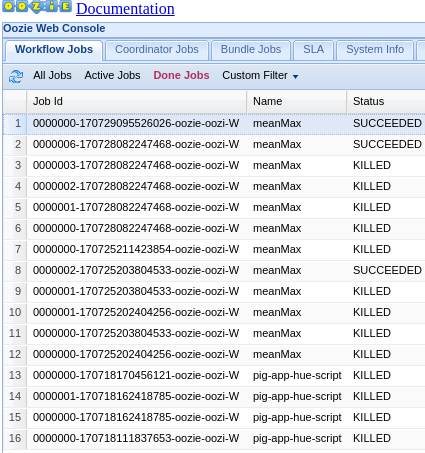
\includegraphics[width=\textwidth, height=5.0in]{fig/06/01}
  \caption{Lista de \textit{jobs} de Oozie ejecutados.}
\end{figure}

\begin{figure}[H]
  \centering
      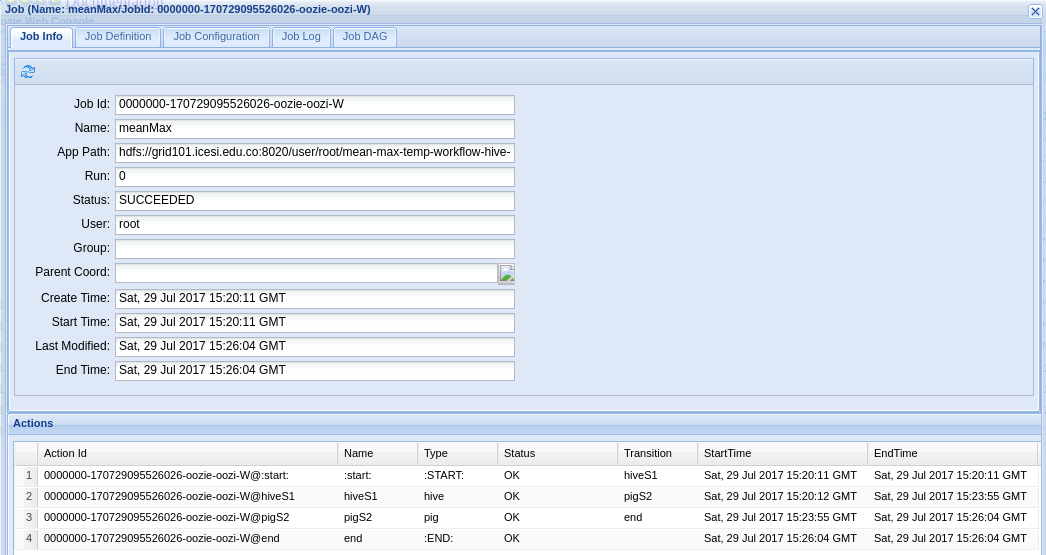
\includegraphics[width=\textwidth, height=5.0in]{fig/06/02}
  \caption{Detalle del \textit{job} de Oozie ejecutado.}
\end{figure}

\begin{figure}[H]
  \centering
      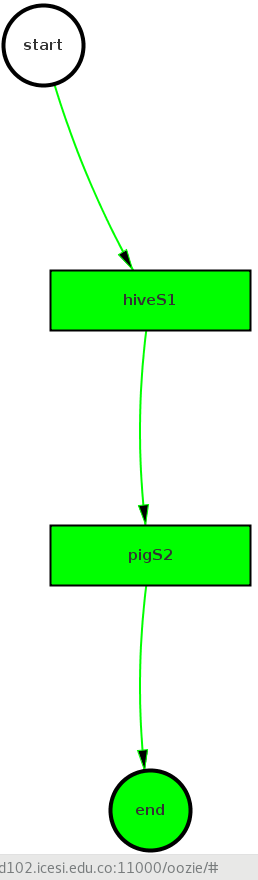
\includegraphics[width=3.0in, height=6.0in]{fig/06/03}
  \caption{Ejecución finalizada, vista desde el grafo acíclico dirigido generado desde la UI del servidor de Oozie.}
\end{figure}